% 2015
% Łukasz Dąbek & Maciej Szeptuch
% II UWr

\documentclass[polish, t,10pt]{beamer}
\usetheme{Antibes}
\usecolortheme{lily}
\setbeamertemplate{footline}[frame number]
\setbeamertemplate{navigation symbols}{}

\usepackage[utf8]{inputenc}
\usepackage{polski}
\usepackage{babel}

\usepackage{multicol}
\usepackage{graphicx}
\usepackage{wrapfig}

%% Kropka po numerze paragrafu, podparagrafu, itp.
\makeatletter
    \renewcommand\@seccntformat[1]{\csname the#1\endcsname.\quad}
    \renewcommand\numberline[1]{#1.\hskip0.7em}
\makeatother

%% Numeracja wzorów
\renewcommand{\theequation}{\arabic{section}.\arabic{equation}}

%% Plan przed każdą sekcją
\AtBeginSection[]
{
    \begin{frame}<beamer>
        \tableofcontents[currentsection]
    \end{frame}
}

%%%%%%%%%%%%%%%%%%%%%%%%%%%%%%%%%%%%%%%%%%%%%%%%%%%%%%%%%%%%%%%%%%%%%%%%%%%%%%%

\title{Wireless link scheduling}
\subtitle{w modelu SINR}
\author{Łukasz Dąbek \& Maciej Szeptuch}
\date{Wrocław, \today}

\begin{document}

\begin{frame}[c]
    \begin{figure}
        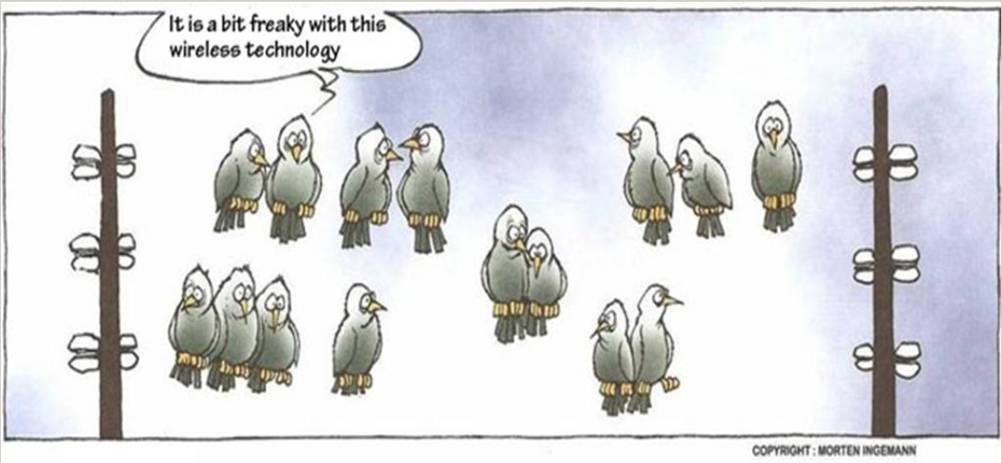
\includegraphics[width=\textwidth]{pictures/obligatory-birds.jpg}
    \end{figure}
\end{frame}

% STRONA TYTUŁOWA
\begin{frame}
    \titlepage
\end{frame}

% PLAN
\begin{frame}
    \frametitle{Plan}
    \tableofcontents
\end{frame}

\def \si {{\color{green}s_i}}
\def \sj {{\color{green}s_j}}
\def \sno {{\color{green}s_{n+1}}}
\def \snt {{\color{green}s_{n+2}}}

\def \ri {{\color{red}r_i}}
\def \rj {{\color{red}r_j}}
\def \rrj {{\color{red}j}}
\def \rno {{\color{red}r_{n+1}}}
\def \rnt {{\color{red}r_{n+2}}}

\def \li {{\color{blue}l_i}}
\def \lj {{\color{blue}l_j}}
\def \lo {{\color{blue}l_1}}
\def \ln {{\color{blue}l_n}}
\def \lno {{\color{blue}l_{n+1}}}
\def \lnt {{\color{blue}l_{n+2}}}
\def \lm {{\color{blue}l_m}}

\def \dii {{\color{cyan}d_{i.i}}}
\def \dij {{\color{cyan}d_{i.j}}}

% Opis
\section{SINR}
\subsection{Model}
    \begin{frame}
        \frametitle{Model}
        \begin{wrapfigure}{R}{0.5\textwidth}
            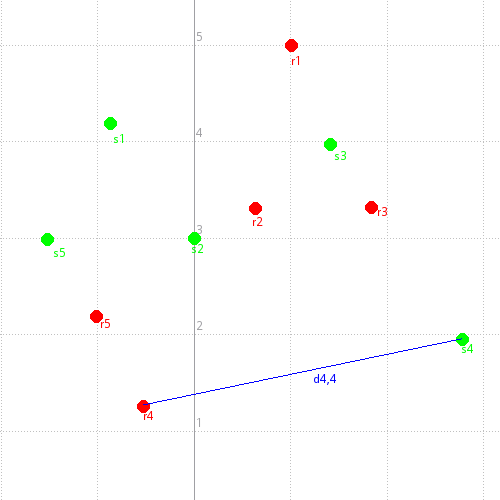
\includegraphics[width=0.5\textwidth]{pictures/model-variables.png}
        \end{wrapfigure}
        Oznaczenia
        \begin{itemize}
            \item $\mathcal{L} = \{\lo, \ldots, \ln\}$ - połączenia
            \item $\li = (\si, \ri)$
            \item $\dij = d(\si, \rj)$
        \end{itemize}
        ~\\
        Założenia
        \begin{itemize}
            \item $\forall_{\si, \rj} \dij \geq 1$
            \item Każdy nadajnik i odbiornik należy do dokładnie jednego połączenia
            \item Jednostkowe obciążenia
        \end{itemize}
    \end{frame}
    \begin{frame}
        \frametitle{Model}
        \begin{wrapfigure}{R}{0.5\textwidth}
            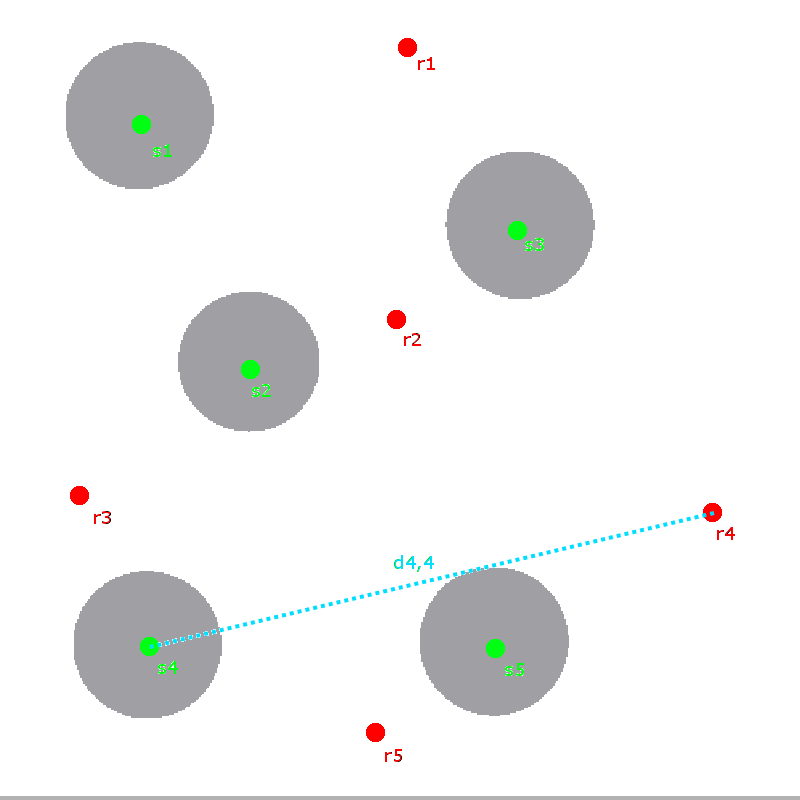
\includegraphics[width=0.5\textwidth]{pictures/model-diagram1.png}
            \caption{$\alpha=2, \beta=1, P=1000$}
        \end{wrapfigure}
        Oznaczenia cd.:
        \begin{itemize}
            \item $P(\si)$ - moc
            \item $\dij^{-\alpha}$ - strata sygnału
            \item $\alpha$ - zazwyczaj $2 \le \alpha \leq 6$
            \item $P_{ii} = P_{\ri}(\si) = P(\si) \cdot \dii^{-\alpha}$
            \item $I_{ji} = I_{\rj}(\si) = P_{\rj}(\si)$ - interferencja
        \end{itemize}
    \end{frame}
    \begin{frame}
        \frametitle{Model}
        \begin{wrapfigure}{R}{0.5\textwidth}
            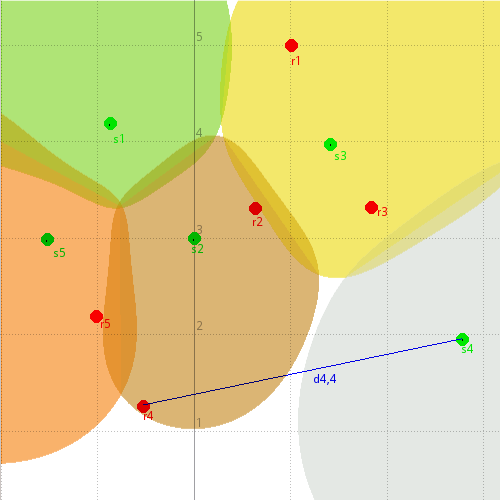
\includegraphics[width=0.5\textwidth]{pictures/model-diagram2.png}
            \caption{$\alpha=2, \beta=0.4, P=1000$}
        \end{wrapfigure}
        Oznaczenia cd.:
        \begin{itemize}
            \item $\mathcal{S}_t = \{\lo, \ldots, \lm\}$ - jeden przedział czasowy
            \item $I_{\ri} = I_{\ri}(S_t) = \sum_{\lj \in S_t, \lj \neq \li} I_{\ri}(\sj)$
            \item $N$ - szum otoczenia
            \item $SINR_{\li} = SINR_{\li}(S_t) = \frac{P_{\ri}(\si)}{I_{\ri} + N}$ - [signal-to-interference-plus-noise-ratio] współczynnik sygnału do szumu i interferencji
        \end{itemize}
    \end{frame}
    \begin{frame}
        \frametitle{Model}
        \begin{wrapfigure}{R}{0.5\textwidth}
            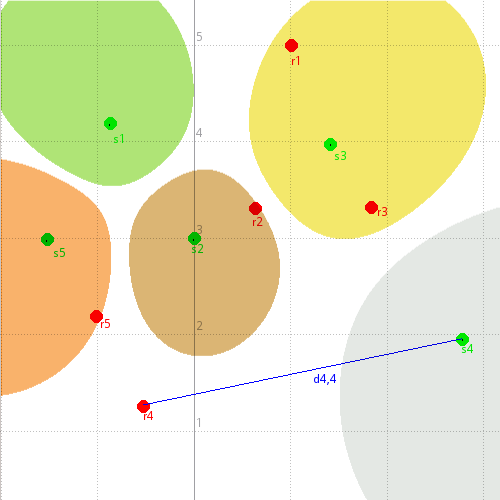
\includegraphics[width=0.5\textwidth]{pictures/model-diagram3.png}
            \caption{$\alpha=2, \beta=1, P=1000000$}
        \end{wrapfigure}
        Oznaczenia cd.:
        \begin{itemize}
            \item $\beta$ - współczynnik odbioru sygnału, zależny od sprzętu
            \item sygnał jest poprawnie odbierany wtw. $SINR_{\li} \geq \beta$
            \item harmonogram $\mathcal{S} = \{\mathcal{S}_1, \ldots, \mathcal{S}_T\}$ jest realizowalny jeśli $\forall_{\mathcal{S}_t \in \mathcal{S}} \forall_{\li \in \mathcal{S}_t} SINR_{\li}(\mathcal{S}_t) \geq \beta$
        \end{itemize}
    \end{frame}
\subsection{Problemy}
    \begin{frame}
        \frametitle{Problemy}
        \begin{wrapfigure}{R}{0.5\textwidth}
            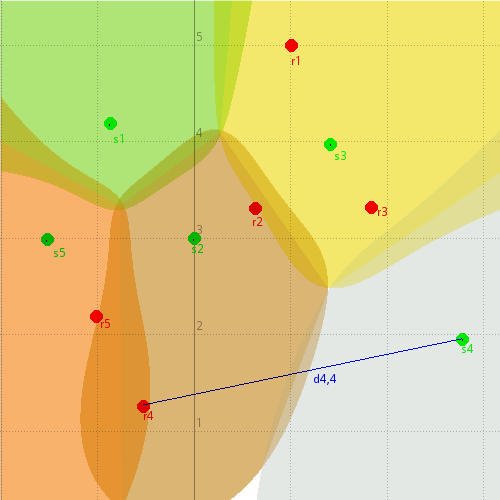
\includegraphics[width=0.5\textwidth]{pictures/model-diagram4.png}
            \caption{$\alpha=2, \beta=0.4, P=1000000$}
        \end{wrapfigure}
        Problemy:
        \begin{itemize}
            \item (Weighted) One-Slot - jak najwięcej połączeń na raz
            \item Multi-Slot - jak najmniej przedziałów
            \item Regulacja mocy - każdy może nadawać z różną mocą
            \item Inne wariacje
        \end{itemize}
    \end{frame}

\begin{frame}[c]
    \begin{figure}
        
\includegraphics[width=\textwidth]{pictures/obligatory-monkey.jpg}
    \end{figure}
\end{frame}

\section{NP-Trudność Multi-Slot}
\subsection{Twierdzenie}
\begin{frame}
    \frametitle{NP-trudność Multi-Slot}
    \begin{definition}[Problem Podziału]
        Mając dany skończony zbiór liczb całkowitych dodatnich określić czy istnieje jego podział na dwa rozłączne podzbiory o równej sumie elementów.
    \end{definition}
    \pause
    \begin{fact}
        Problem Podziału jest NP-zupełny.
    \end{fact}
    \pause
    \begin{theorem}
        Problem Multi-Slot w modelu SINR jest NP-trudny.
    \end{theorem}
    \pause
    \begin{block}{Dowód}
        Pokażemy wielomianową redukcje Problemu Podziału do problemu Multi-Slot w modelu SINR.
    \end{block}
\end{frame}
\subsection{Idea dowodu}
\begin{frame}
    \frametitle{Idea dowodu}
    Na podstawie zbioru liczb z Problemu Podziału stworzymy instancje Multi-Slot o następujących własnościach:
    \begin{itemize}
        \item Połączenia będą odpowiadać liczbom z Problemu Podziału
        \item Poza dodatkowymi dwoma, które będą służyć za strażników
        \item Wszystkie połączenia $\lj$ niebędące strażnikami będą w punkcie $(0, 0)$ wywoływać interferencje równą $i_j$
        \item Strażnicy będą mieć odbiorniki w punkcie $(0, 0)$ i nadajniki w takiej odległości aby moc połączenia wynosiła $\frac{\sigma}{2}$
        \item Wszystkie $\lj$ dla $j \leq n$ są realizowalne w jednym przedziale czasowym
    \end{itemize}
\end{frame}
\subsection{Dowód}
\begin{frame}
    \frametitle{NP-trudność}
    \begin{theorem}
        Problem Multi-Slot w modelu SINR jest NP-trudny.
    \end{theorem}
    \begin{wrapfigure}{R}{0.5\textwidth}
        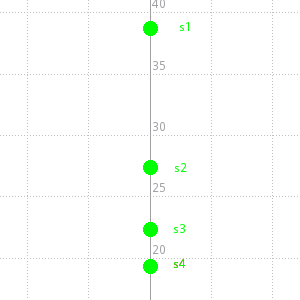
\includegraphics[width=0.5\textwidth]{pictures/np-placement1.png}
    \end{wrapfigure}
    \begin{block}{Oznaczenia}
        \begin{itemize}
            \item $\mathcal{I} = \{i_1, \ldots. i_n\}$ - zbiór liczb z Problemu Podziału o sumie $\sigma$
            \item BSO wszystkie elementy $\mathcal{I}$ są różne
            \item $\mathcal{L} = \{\lo, \ldots, \lnt\}$ - zbiór połączeń dla Multi-Slota
            \item $\forall_{1 \leq j \leq n} pos(\sj) = \Big(0, \big(\frac{P}{i_j}\big)^\frac{1}{\alpha}\Big)$ - pozycja nadajników
        \end{itemize}
    \end{block}
\end{frame}
\begin{frame}
    \frametitle{NP-trudność}
    \begin{wrapfigure}{R}{0.5\textwidth}
        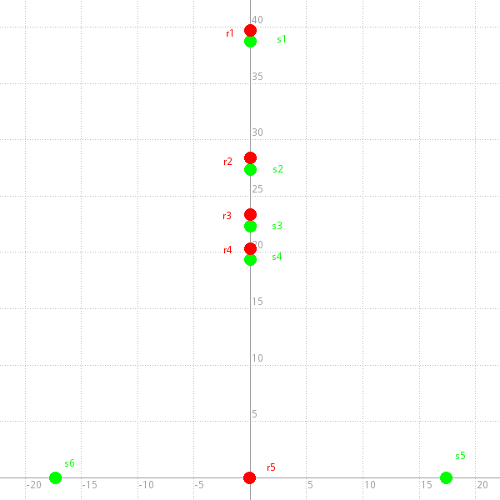
\includegraphics[width=0.5\textwidth]{pictures/np-placement2.png}
    \end{wrapfigure}
    \begin{block}{Oznaczenia cd.}
        \begin{itemize}
            \item $d_{min} = P^\frac{1}{\alpha}\cdot\frac{(i_{max}-1)^\frac{-1}{\alpha}-(i_{max})^\frac{-1}{\alpha}}{1+(n\beta)^\frac{1}{\alpha}}$
            \item $\forall_{1 \leq j \leq n} pos(\rj) = pos(\sj) + (0, d_{min})$ - pozycja odbiorników
            \item $pos(\rno) = pos(\rnt) = (0, 0)$
            \item $pos(\sno) = \Big(\big(\frac{2P}{\beta\sigma}\big)^\frac{1}{\alpha}, 0\Big)$
            \item $pos(\snt) = \Big(-\big(\frac{2P}{\beta\sigma}\big)^\frac{1}{\alpha}, 0\Big)$
        \end{itemize}
    \end{block}
\end{frame}
\begin{frame}
    \frametitle{NP-trudność}
    \begin{lemma}
        Niech $\mathcal{L}_i = \{\lj: 1 \leq j \leq n + 1, i \neq j\}$.\\
        Dla każdego $i \leq n$ kiedy $\li$ jest zaplanowany wraz z elementami $\mathcal{L}_i$ wartość $SINR_\li \ge \beta$,
        $$
            SINR_\li(\mathcal{L}_i) = \frac{P_{ii}}{\sum_{\lj \in \mathcal{L}_i} I_{ij}} > \beta
        $$
    \end{lemma}
\end{frame}
\begin{frame}
    \centering
    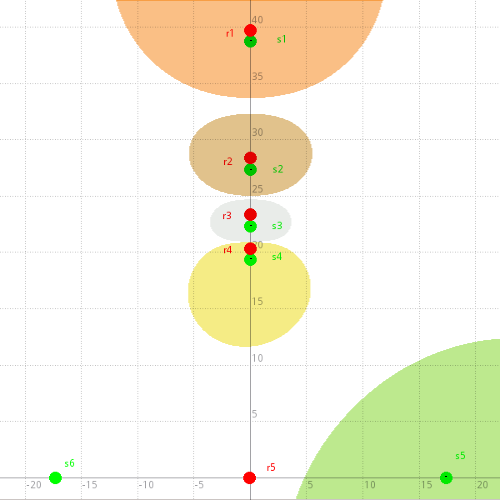
\includegraphics[width=0.75\textwidth]{pictures/np-placement3.png}
\end{frame}
\begin{frame}
    \frametitle{NP-trudność}
    \begin{lemma}
        Niech $\mathcal{L}_i = \{\lj: 1 \leq j \leq n + 1, i \neq j\}$.\\
        Dla każdego $i \leq n$ kiedy $\li$ jest zaplanowany wraz z elementami $\mathcal{L}_i$ wartość $SINR_\li \ge \beta$,
        $$
            SINR_\li(\mathcal{L}_i) = \frac{P_{ii}}{\sum_{\lj \in \mathcal{L}_i} I_{ij}} > \beta
        $$
    \end{lemma}
    \pause
    \begin{block}{Wniosek}
        Jeśli zapomnimy o jednym z $\lno, \lnt$ wszystkie pozostałe połączenia są realizowalne w jednym przedziale czasowym.
    \end{block}
\end{frame}
\begin{frame}
    \frametitle{NP-trudność}
    Jeśli mamy rozwiązanie Problemu Podziału to mamy też Multi-Slota w 2 przedziałach czasowych.
    \begin{block}{Uzasadnienie}
        Dostajemy $\mathcal{I}_1, \mathcal{I}_2 \subset \mathcal{I}$ takie że sumują się do $\sigma/2$. Przydzielamy wszystkie $\lj$ takie że $i_j \in \mathcal{I}_1$ to pierwszego przedziału wraz z $\lno$ a pozostałe do drugiego.
    \end{block}
    \pause
    \begin{block}{Obserwacja}
        Moc sygnału na odbiorniku $\rno$: $P_\rno(\sno) = \frac{\beta\sigma}{2}$.
    \end{block}
    \pause
    \begin{block}{Obserwacja}
        Moc interferencji na odbiorniku $\rno$: $I_\rno(\sj) = i_j$. Co daje całkowitą interferencje $I_\rno = \frac{\sigma}{2}$.
    \end{block}
\end{frame}
\begin{frame}
    \frametitle{NP-trudność}
    \centering
    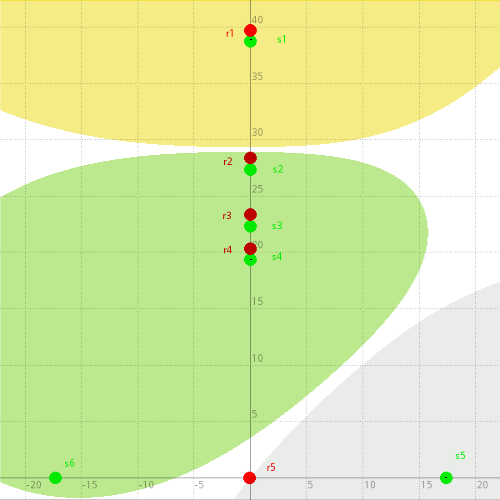
\includegraphics[width=0.5\textwidth]{pictures/np-ok1.png}
    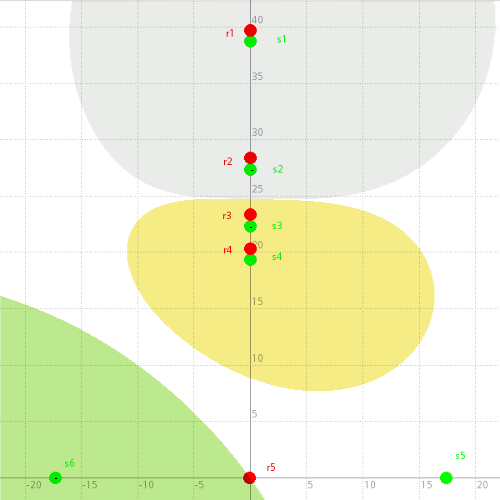
\includegraphics[width=0.5\textwidth]{pictures/np-ok2.png}
\end{frame}
\begin{frame}
    \frametitle{NP-trudność}
    Jeśli mamy rozwiązanie Problemu Podziału to mamy też Multi-Slota w 2 przedziałach czasowych.
    \begin{block}{Uzasadnienie}
        Dostajemy $\mathcal{I}_1, \mathcal{I}_2 \in \mathcal{I}$ takie że sumują się do $\sigma/2$. Przydzielamy wszystkie $\lj$ takie że $i_j \in \mathcal{I}_1$ to pierwszego przedziału wraz z $\lno$ a pozostałe do drugiego.
    \end{block}
    \begin{block}{Obserwacja}
        Moc sygnału na odbiorniku $\rno$: $P_\rno(\sno) = \frac{\beta\sigma}{2}$.
    \end{block}
    \begin{block}{Obserwacja}
        Moc interferencji na odbiorniku $\rno$: $I_\rno(\sj) = i_j$. Co daje całkowitą interferencje $I_\rno = \frac{\sigma}{2}$.
    \end{block}
    \pause
    \begin{block}{Wniosek}
        $SINR_\rno \geq \beta$
    \end{block}
\end{frame}
\begin{frame}
    \frametitle{NP-trudność}
    Jeśli nie ma rozwiązania Problemu Podziału to nie da się rozwiązać Multi-Slota w 2 przedziałach czasowych.
    \begin{block}{Uzasadnienie}
        Problem Podziału nie ma rozwiązania, a to znaczy że dla każdego podziału jeden ze zbiorów ma sumę większą niż $\sigma/2$.
    \end{block}
    \pause
    \begin{block}{Obserwacja}
        Dla każdego podziału $\li$ na dwa przedziały czasowe całkowita interferencja w $(0, 0)$ dla jednego z nich będzie większa niż $\sigma/2$ co zakłóci odbiór sygnału.
    \end{block}
\end{frame}
\begin{frame}
    \frametitle{NP-trudność}
    \centering
    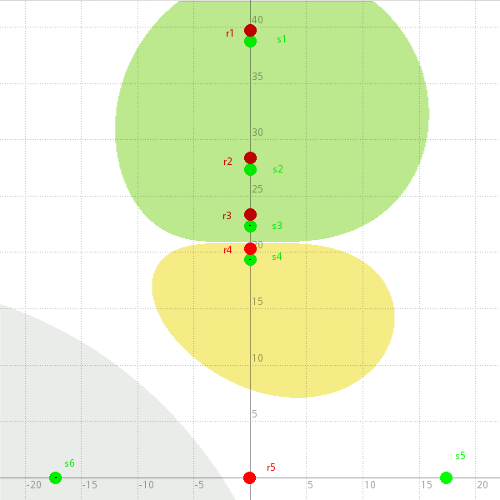
\includegraphics[width=0.5\textwidth]{pictures/np-error1.png}
    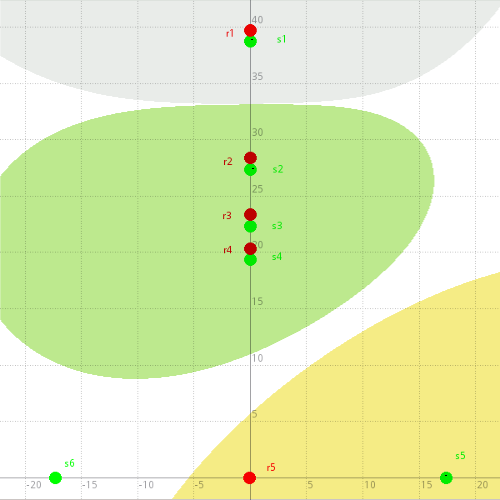
\includegraphics[width=0.5\textwidth]{pictures/np-error2.png}
\end{frame}
\begin{frame}
    \frametitle{NP-trudność}
    Jeśli nie ma rozwiązania Problemu Podziału to nie da się rozwiązać Multi-Slota w 2 przedziałach czasowych.
    \begin{block}{Uzasadnienie}
        Problem Podziału nie ma rozwiązania, a to znaczy że dla każdego podziału jeden ze zbiorów ma sumę większą niż $\sigma/2$.
    \end{block}
    \begin{block}{Obserwacja}
        Dla każdego podziału $\li$ na dwa przedziały czasowe całkowita interferencja w $(0, 0)$ dla jednego z nich będzie większa niż $\sigma/2$ co zakłóci odbiór sygnału.
    \end{block}
    \pause
    \begin{block}{Wniosek}
        Pokazaliśmy redukcję wielomianową z Problemu Podziału, który jest NP-zupełny, do Multi-Slot z czego wynika że Multi-Slot jest NP-trudny.
    \end{block}
\end{frame}

\begin{frame}[c]
    \begin{figure}
        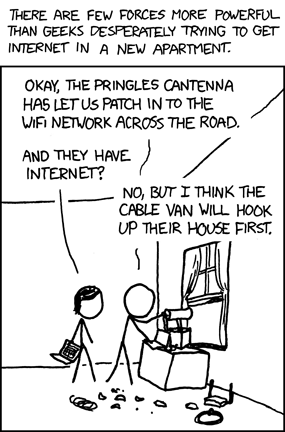
\includegraphics[width=0.5\textwidth]{pictures/obligatory-xkcd.png}
    \end{figure}
\end{frame}

\section{Aproksymacja One-Slot}
\begin{frame}
    \frametitle{Problem}
        Czy istnieje algorytm rozwiązujący One-Slot Scheduling działający w czasie wielomianowym,
        który daje wynik gorszy tylko o stały czynnik od optymalnego?
        \pause
        \vfill
        Tak.
\end{frame}

\subsection{Wiadomości wstępne}
\begin{frame}
    \frametitle{Notacja}
    \begin{itemize}
        \item Wpływ: $a_v(S) = \eta_v \sum_{w \in S} \frac{I_{wv}}{P_{vv}}$
        \item Łatwość zakłócenia: $\eta_v = \frac{1}{\frac{1}{\beta} - \frac{N}{P_{vv}}}$
        \item $OPT_p$ - rozwiązanie, w którym dla każdego połączenia $v$: $a_v(OPT_p) \le p^{-\alpha}$
    \end{itemize}
\end{frame}

\begin{frame}
    \frametitle{Własności wpływu}
    \begin{definition}
        $a_v(S) = \eta_v \sum_{w \in S} \frac{I_{wv}}{P_{vv}}$\\
        $\eta_v = \frac{1}{\frac{1}{\beta} - \frac{N}{P_{vv}}}$
    \end{definition}
    \begin{lemma}
        Jeśli $S_1$ i $S_2$ są rozłącznymi zbiorami połączeń, to $a_v(S_1 \cup S_2) = a_v(S_1) + a_v(S_2)$.
    \end{lemma}
    \begin{lemma}
        Zestaw połączeń $S$ jest realizowalny wtedy i tylko wtedy, gdy dla każdego $v$ zachodzi:
        $a_v(S) \le 1$.
    \end{lemma}
\end{frame}

\begin{frame}
    \frametitle{$q$-bliskość}
    \begin{definition}
        Mówimy, że połączenie $w$ jest $q$-blisko połączenia $v$ jeśli $d_{wv} \ge q \eta_v^{1/\alpha} d_{vv}$.
        Równoważnie: $a_v(w) = a_v(\{w\}) \ge q^{-\alpha}$.
    \end{definition}

    \begin{definition}
        Zbiór $S$ jest $q$-rozproszony, jeżeli dla każdej pary połączeń $v$, $w$ w $S$ połączenie $w$ nie jest $q$-blisko połączenia $v$.
    \end{definition}
\end{frame}

\begin{frame}
    \frametitle{Algorytm}
    Niech $\lambda$ będzie pewną (dużą) stałą, do ustalenia później.
    \begin{itemize}
        \item Posortuj połączenia w kolejności rosnącej długości: $l_1, l_2, \cdots, l_n$.
        \item Niech $S = \varnothing$.
        \item Dla połączenia $l_i = l_1, l_2, \cdots, l_n$:
        \begin{itemize}
            \item Jeśli $a_{l_i}(S) \le \lambda^{-\alpha}$ dodaj $l_i$ do $S$.
        \end{itemize}
        \item Zwróć $S$.
    \end{itemize}
    \pause
    \vfill
    \begin{itemize}
        \item Czy zwrócony zbiór jest realizowalny?
        \pause
        \item Czy zwrócony zbiór jest tylko o stały czynnik większy od optymalnego?
    \end{itemize}
\end{frame}

\subsection{Poprawność algorytmu}
\begin{frame}
    \frametitle{Rozproszenie rozwiązania}
    \begin{lemma}
        Zwrócony zbiór połączeń jest $(\lambda - 2)$-rozproszony.
    \end{lemma}
    Dowód: nierówność trójkąta. \\
    \centering
    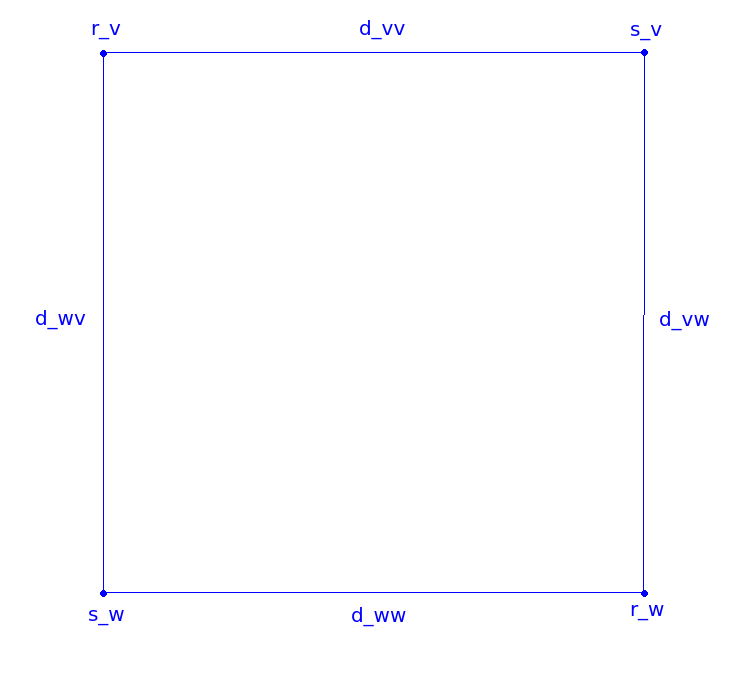
\includegraphics[width=0.6\textwidth]{pictures/triangle-inequality.png}
\end{frame}

\begin{frame}
    \frametitle{Lemat o pierścieniach}
    \begin{lemma}
        Niech $S$ będzie $\delta$-rozproszony i niech $v$ będzie najkrótszym połączeniem w $S$. Wtedy:
        \begin{equation*}
            a_v(S) \lesssim \delta^{-\alpha}
        \end{equation*}
    \end{lemma}
    \centering
    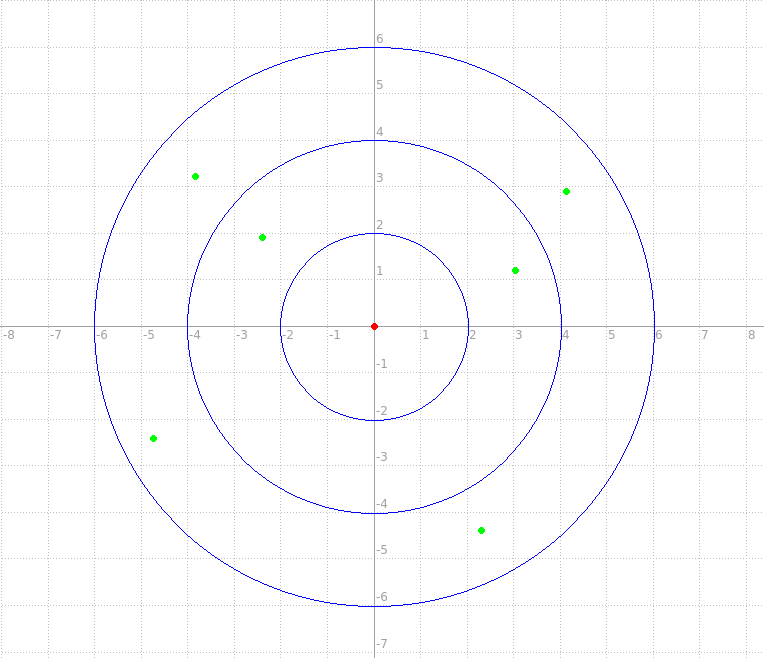
\includegraphics[width=0.6\textwidth]{pictures/rings.png}
\end{frame}

\begin{frame}
    \frametitle{Lemat o pierścieniach}
    \begin{lemma}
        Jedyny odbiornik w promieniu $\delta \eta_v^{1/\alpha} d_{vv}$ od nadajnika $r_w$ to
        co najwyżej $s_w$.
    \end{lemma}
    \pause
    \begin{lemma}
        Dookoła każdego odbiornika nie ma innych odbiorników w promieniu $d_{vv}(\delta\eta_v^{1/\alpha} - 1)/2$.
    \end{lemma}
\end{frame}

\begin{frame}
    \frametitle{Lemat o pierścieniach}
    \centering
    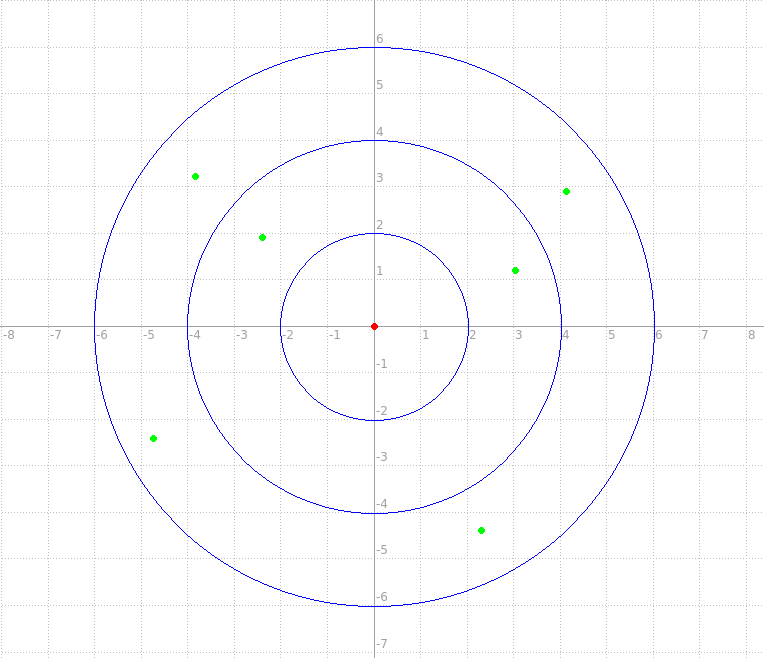
\includegraphics[width=0.7\textwidth]{pictures/rings.png}
\end{frame}

\begin{frame}
    \frametitle{Lemat o pierścieniach}
    \centering
    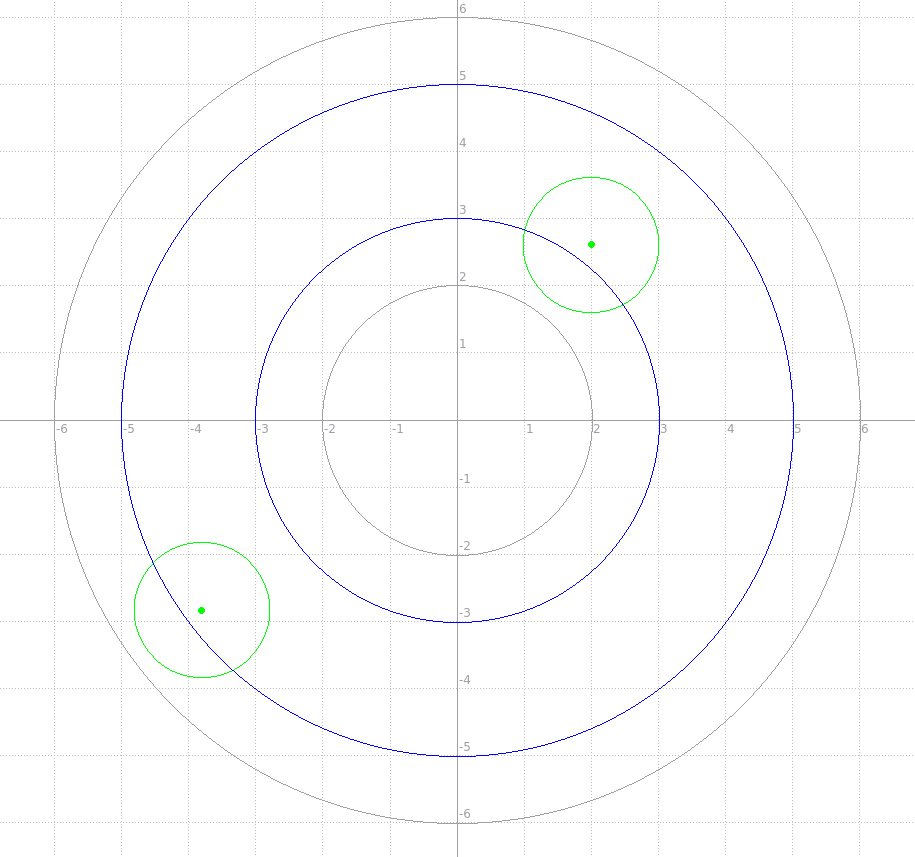
\includegraphics[width=0.7\textwidth]{pictures/bigger-rings.png}
\end{frame}

\begin{frame}
    \frametitle{Lemat o pierścieniach}
    \centering
    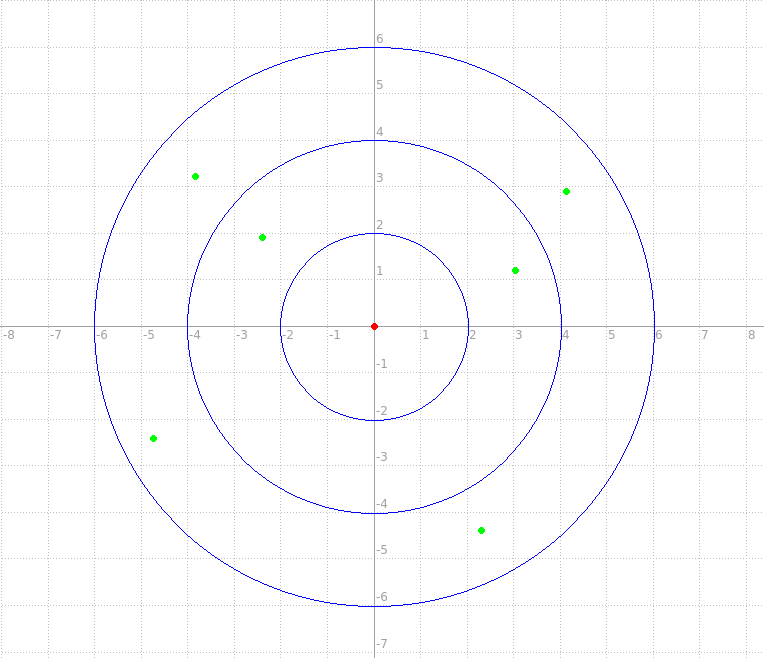
\includegraphics[width=0.7\textwidth]{pictures/rings.png}
\end{frame}

\begin{frame}
    \frametitle{Poprawność rozwiązania}
    \begin{lemma}
        Rozwiązanie zwracane przez algorytm zachłanny jest poprawne (tj. spełnialne w sensie SINR).
    \end{lemma}
    Dla ustalonego połączenia $l_v$ dzielimy zbiór połączeń na krótsze niż $l_v$ i dłuższe - odpowiednio $S^{-}$ i $S^{+}$.
    Z definicji algorytmu mamy $a_{l_v}(S^{-}) \le \lambda^{-\alpha}$. Z lematu o pierścieniach mamy
    $a_{l_v}(S^{+}) \lesssim (\lambda - 2)^{-\alpha}$. \\
    Zatem dobierając odpowiednio duże $\lambda$ zapewniamy, że $a_{l_v}(S) \le 1/2$.
\end{frame}


\subsection{Jakość rozwiązania}
\begin{frame}
    \frametitle{Lemat o niebieskich punktach}
    \begin{definition}
        Rozważmy dwa skończone zbiory punktów $\mathcal{R}, \mathcal{B}$ nazywane odpowiednio czerwonymi i
        niebieskimi. Mówimy, że punkt $b \in \mathcal{B}$ jest q-niebiesko-dominujący, jeżeli każde koło
        o środku w $b$ zawiera przynajmniej q razy więcej punktów niebieskich niż czerwonych.
    \end{definition}
    \vfill
    \begin{lemma}
        Jeżeli $|\mathcal{B}| \ge 6q|\mathcal{R}|$, to istnieje punkt q-niebiesko-dominujący.
    \end{lemma}
\end{frame}

\begin{frame}
    \frametitle{Lemat o niebieskich punktach}
    \centering
    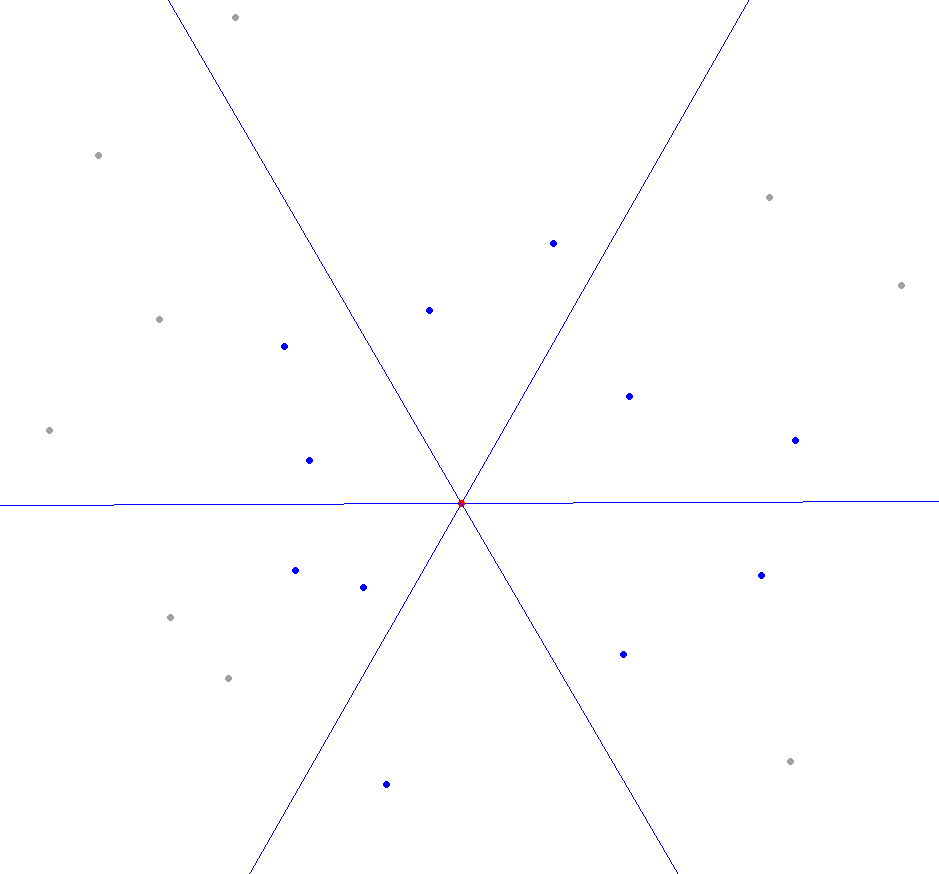
\includegraphics[width=0.7\textwidth]{pictures/blue-dominant-1.png}
\end{frame}

\begin{frame}
    \frametitle{Lemat o niebieskich punktach}
    \centering
    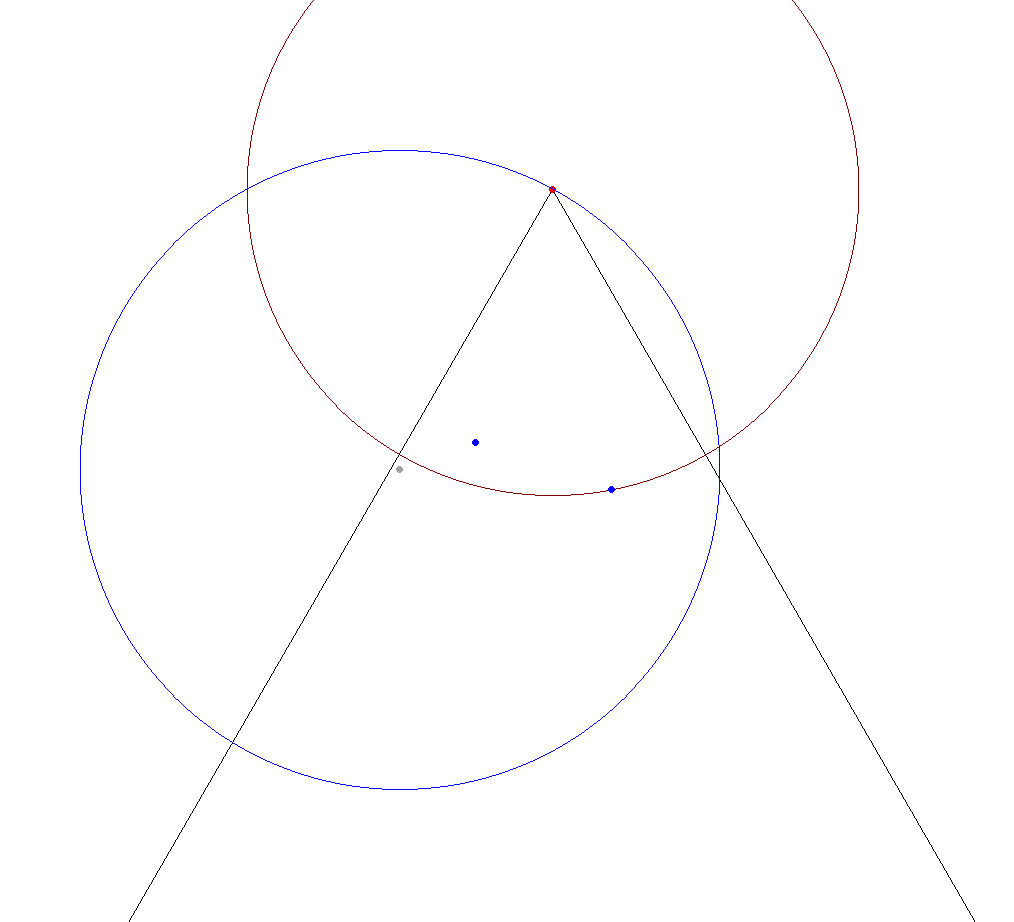
\includegraphics[width=0.7\textwidth]{pictures/blue-dominant-2.png}
\end{frame}

\begin{frame}
    \frametitle{Porównanie jakości rozwiązania z $OPT_p$}
    \begin{lemma}
        Niech $S$ będzie rozwiązaniem wyprodukowanym przez algorytm zachłanny. Wtedy:
        $|S| \lesssim |OPT_{\lambda^{\alpha}}|$.
    \end{lemma}
\end{frame}

\begin{frame}
    \frametitle{$|OPT_p| \lesssim |OPT|$}
    \begin{lemma}
        $|OPT_p| \le \lceil (2p)^2 \rceil |OPT|$
    \end{lemma}
\end{frame}

%\section{Wypukłość obszarów SINR}
\section{Do zrobienia}
\end{document}
